\documentclass[a4paper,12pt]{article}

% Some basic packages
\usepackage[utf8]{inputenc}
\usepackage[T1]{fontenc}
\usepackage{textcomp}
\usepackage[english]{babel}
\usepackage{url}
\usepackage{graphicx}
\usepackage{float}
\usepackage{booktabs}
% \usepackage{enumitem}
\usepackage{enumerate}
\usepackage[colorlinks]{hyperref}

\pdfminorversion=7

% Don't indent paragraphs, leave some space between them
\usepackage{parskip}
\usepackage{changepage}

% Hide page number when page is empty
\usepackage{emptypage}
\usepackage{subcaption}
\usepackage{multicol}
\usepackage[dvipsnames]{xcolor}

% Other font I sometimes use.
% \usepackage{cmbright}

% Math stuff
\usepackage{amsmath, amsfonts, mathtools, amsthm, amssymb}

% Add this line to make equation numbering follow section
\numberwithin{equation}{section}

% Fancy script capitals
\usepackage{mathrsfs}
\usepackage{cancel}
% Bold math
\usepackage{bm}
% Some shortcuts
\newcommand\N{\ensuremath{\mathbb{N}}}
\newcommand\R{\ensuremath{\mathbb{R}}}
\newcommand\Z{\ensuremath{\mathbb{Z}}}
\renewcommand\O{\ensuremath{\emptyset}}
\newcommand\Q{\ensuremath{\mathbb{Q}}}
\newcommand\C{\ensuremath{\mathbb{C}}}

% Easily typeset systems of equations (French package)
\usepackage{systeme}

% Put x \to \infty below \lim
\let\svlim\lim\def\lim{\svlim\limits}

%Make implies and impliedby shorter
\let\implies\Rightarrow
\let\impliedby\Leftarrow
\let\iff\Leftrightarrow
% \let\epsilon\varepsilon

% COURSE SPECIFICS
% GRIFFITHS
\ifdefined\pdfliteral
    \let\griffPdfliteral\pdfliteral
\else \def\griffPdfliteral#1{\special{pdf: literal #1}} \fi

\newcommand\griffr[1][2]{\leavevmode\hbox{\kern1pt\vbox to1ex{}\griffPdfliteral{%
    q 1 J .27 0 0 .27 0 0 cm #1 w
    0 2 m
    0 2 8.1 9.7 9.2 13.2 c
    10.4 16.8 8.4 15.4 8 14.7 c
    7.6 14 6.8 12.6 12 13 c
    17 13.5 14.5 7.8 13.7 6 c
    12.8 4.3 10.3 1.2 11.4 .2 c
    12.6 -.7 18.8 3.6 18.8 3.6 c
    18.8 3.6 l S Q
}\kern6pt}}
\newcommand\hatgriffr{\skew3\hat{\griffr[4]}}

% Add \contra symbol to denote contradiction
\usepackage{stmaryrd} % for \lightning
\newcommand\contra{\scalebox{1.5}{$\lightning$}}

% \let\phi\varphi

% Command for short corrections
% Usage: 1+1=\correct{3}{2}

\definecolor{correct}{HTML}{009900}
\newcommand\correct[2]{\ensuremath{\:}{\color{red}{#1}}\ensuremath{\to }{\color{correct}{#2}}\ensuremath{\:}}
\newcommand\green[1]{{\color{correct}{#1}}}

% horizontal rule
\newcommand\hr{
    \noindent\rule[0.5ex]{\linewidth}{0.5pt}
}

% hide parts
\newcommand\hide[1]{}

% si unitx
\usepackage{siunitx}
\sisetup{locale = FR}

% Environments
\makeatother
% For box around Definition, Theorem, ...
% \usepackage{mdframed}
\usepackage[framemethod=TikZ]{mdframed}

% Custom command to draw a rectangular border around an equation
\setlength{\fboxsep}{5pt}  % Adjust padding inside the box
\usepackage{empheq}
\newcommand*\widefbox[1]{\fbox{\hspace{1em}#1\hspace{1em}}}

\usepackage{environ}  % This package allows for easier custom environment definitions

% Define the custom environment
\NewEnviron{framed}{%
  \begin{empheq}[box=\fbox]{align}
  \BODY
  \end{empheq}
}
% Custom environment to box align equations
% \newenvironment{boxedalign}
%   {\begin{empheq}[box=\fbox]{align}}
%   {\end{align}\end{empheq}}

\newtheorem{thm}{Theorem}[subsection]
\newtheorem{defi}[thm]{Definition}
\newtheorem{lem}[thm]{Lemma}
\newtheorem{ret}{Correction}


\newtheorem*{term}{Terminology}
\newtheorem*{key}{Keywords and Related Concepts}
\newtheorem{lign}[thm]{Equation}
\newtheorem{law}[thm]{Law / Principle}

\usepackage{mathtools}
\DeclarePairedDelimiter\bra{\langle}{\rvert}
\DeclarePairedDelimiter\ket{\lvert}{\rangle}
\DeclarePairedDelimiterX\braket[2]{\langle}{\rangle}{#1\,\delimsize\vert\,\mathopen{}#2}


% \newcounter{theo}[section]
% \renewcommand{\thetheo}{\arabic{section}.\arabic{theo}}

% \mdfsetup{skipabove=1em,skipbelow=0em}
% \theoremstyle{definition}
% \newmdtheoremenv[nobreak=true]{definition}{Definition}
% \newmdtheoremenv[nobreak=true]{theorem}{Theorem}
% \newmdtheoremenv[nobreak=true]{corollary}{Corollary}
% \newmdtheoremenv[nobreak=true]{lemma}{Lemma}

% \newtheorem*{observation}{Observation}
% \newtheorem*{property}{Property}
% \newtheorem*{postulate}{Postulate}
% \newtheorem*{conclusion}{Conlusion}
% \newtheorem*{repitition}{Repitition}
% \newtheorem*{example}{Example}
% \newtheorem*{question}{Question}
% \newtheorem*{intuition}{Intuition}

% End example and intermezzo environments with a small diamond (just like proof
% environments end with a small square)
% \usepackage{etoolbox}
% \AtEndEnvironment{example}{\null\hfill$\diamond$}%
% \AtEndEnvironment{repitition}{\null\hfill$\diamond$}%
% \AtEndEnvironment{opmerking}{\null\hfill$\diamond$}%

% Fix some spacing
% http://tex.stackexchange.com/questions/22119/how-can-i-change-the-spacing-before-theorems-with-amsthm
\makeatletter
\def\thm@space@setup{%
  \thm@preskip=\parskip \thm@postskip=0pt
}


% Exercise 
% Usage:
% \oefening{5}
% \suboefening{1}
% \suboefening{2}
% \suboefening{3}
% gives
% Oefening 5
%   Oefening 5.1
%   Oefening 5.2
%   Oefening 5.3
\newcommand{\exercise}[1]{%
    \def\@exercise{#1}%
    \subsection*{Exercise #1}
}

\newcommand{\subexercise}[1]{%
    \subsubsection*{Exercise \@exercise.#1}
}

\usepackage{xcolor}
\newcommand{\textred}[1]{\textcolor{red}{#1}}

% \lecture starts a new lecture (les in dutch)
%
% Usage:
% \lecture{1}{di 12 feb 2019 16:00}{Inleiding}
%
% This adds a section heading with the number / title of the lecture and a
% margin paragraph with the date.

% I use \dateparts here to hide the year (2019). This way, I can easily parse
% the date of each lecture unambiguously while still having a human-friendly
% short format printed to the pdf.

\usepackage{xifthen}
\def\testdateparts#1{\dateparts#1\relax}
\def\dateparts#1 #2 #3 #4 #5\relax{
    \marginpar{\small\textsf{\mbox{#1 #2 #3 #5}}}
}

\def\@lecture{}%
\newcommand{\lecture}[3]{
    \ifthenelse{\isempty{#3}}{%
        \def\@lecture{Lecture #1}%
    }{%
        \def\@lecture{Lecture #1: #3}%
    }%
    \subsection*{\@lecture}
    \marginpar{\small\textsf{\mbox{#2}}}
}

\def\@chapter{}%
\newcommand{\chapter}[3]{
    \ifthenelse{\isempty{#3}}{%
        \def\@chapter{Chapter #1}%
    }{%
        \def\@chapter{Chapter #1: #3}%
    }%
    \subsection*{\@chapter}
    \marginpar{\small\textsf{\mbox{#2}}}
}

\def\@week{}%
\newcommand{\week}[3]{
    \ifthenelse{\isempty{#3}}{%
        \def\@week{Uge #1}%
    }{%
        \def\@week{Uge #1: #3}%
    }%
    \subsection*{\@week}
    \marginpar{\small\textsf{\mbox{#2}}}
}

% These are the fancy headers
% \usepackage{fancyhdr}
% \pagestyle{fancy}

% LE: left even
% RO: right odd
% CE, CO: center even, center odd
% My name for when I print my lecture notes to use for an open book exam.
% \fancyhead[LE,RO]{Gilles Castel}

% \setlength{\headheight}{5pt}

% % \fancyhead[R]{\@lecture} % Right odd,  Left even
% \fancyfoot[R]{\thepage}  % Right odd,  Left even
% \fancyfoot[C]{\leftmark}     % Center

\makeatother

% Todonotes and inline notes in fancy boxes
\usepackage{todonotes}
\usepackage{tcolorbox}

% Make boxes breakable
\tcbuselibrary{breakable}

% Usage: 
% \begin{correction}
%     Lorem ipsum dolor sit amet, consetetur sadipscing elitr, sed diam nonumy eirmod
%     tempor invidunt ut labore et dolore magna aliquyam erat, sed diam voluptua. At
%     vero eos et accusam et justo duo dolores et ea rebum. Stet clita kasd gubergren,
%     no sea takimata sanctus est Lorem ipsum dolor sit amet.
% \end{correction}
\newenvironment{correction}{\begin{tcolorbox}[
    arc=0mm,
    colback=white,
    colframe=green!60!black,
    title=Correction,
    fonttitle=\sffamily,
    breakable
]}{\end{tcolorbox}}

% Same as 'correction' but color of box is different
\newenvironment{note}{\begin{tcolorbox}[
    arc=0mm,
    colback=white,
    colframe=white!60!black,
    title=Note,
    fonttitle=\sffamily,
    breakable
]}{\end{tcolorbox}}


% Figure support as explained in my blog post.
\usepackage{import}
\usepackage{xifthen}
\usepackage{pdfpages}
\usepackage{transparent}
\newcommand{\incfig}[1]{%
    \def\svgwidth{\columnwidth}
    \import{./figures/}{#1.pdf_tex}
}

% Fix some stuff
% %http://tex.stackexchange.com/questions/76273/multiple-pdfs-with-page-group-included-in-a-single-page-warning
\pdfsuppresswarningpagegroup=1


% My name
\author{Erik Bach Ryhl}

\graphicspath{{./figs/}}

%--------------------------
% PACKAGES
%--------------------------
\usepackage[utf8]{inputenc}
\usepackage[T1]{fontenc}
\usepackage{amsmath, amssymb, amsfonts}
\usepackage{geometry}
\usepackage{enumitem}
\usepackage{xcolor}
\usepackage{hyperref}
\usepackage{graphicx}
\usepackage{titlesec}
\usepackage{fancyhdr}
\usepackage[normalem]{ulem}

%--------------------------
% PAGE SETUP
%--------------------------
\geometry{margin=1in}
\pagestyle{fancy}
\fancyhf{}
\rhead{\thepage}
\lhead{Learning Journal}

%--------------------------
% SECTION FORMATTING
%--------------------------
\titleformat{\section}[block]{\large\bfseries}{Session \thesection:}{1em}{}
\titleformat{\subsection}[block]{\bfseries}{\thesubsection}{1em}{}
\setcounter{secnumdepth}{2}

%--------------------------
% CUSTOM ENVIRONMENTS
%--------------------------
\newenvironment{deff}[1][Definition]{\par\vspace{1em}\noindent\textbf{#1.}\hspace{0.5em}}{\par\vspace{0.1em}}

\newenvironment{rem}[1][Remark]{\par\vspace{1em}\noindent\textit{#1.}\hspace{0.5em}\begingroup\itshape}{\endgroup\par\vspace{0.1em}}

% Explanation of the custom environment:
% 1. \newenvironment{definition}[1][Definition]: This creates a new environment named "definition" with an optional argument. The default title is "Definition."
% 2. \par\vspace{1em}: Adds vertical space before the environment begins.
% 3. \noindent\textbf{#1.}: Formats the title (e.g., "Definition.") as bold text.
% 4. \hspace{0.5em}: Adds a small space between the title and the definition text.
% 5. The closing curly braces define the formatting after the environment ends, including vertical spacing.


%--------------------------
% DOCUMENT
%--------------------------
\begin{document}

\begin{center}
    {\Huge \textbf{Learning Journal}} \\
    \vspace{0.5em}
    {\large Organized by Sessions with Topic Summaries}
\end{center}
\vspace{1em}
\hrule
\vspace{2em}

%--------------------------
% TEMPLATE STRUCTURE
%--------------------------
\section*{Instructions}
\begin{itemize}
    \item Use this document to track your learning sessions.
    \item Each session entry should include: \begin{enumerate}
        \item Topics covered (briefly).
        \item Key insights or definitions.
        \item Problems attempted (with references or solutions if necessary).
        \item Questions or areas for follow-up.
    \end{enumerate}
    \textit{Make Anki flashcards of whatever makes sense. Even topics if you'd like, just to leverage their spaced repitition algorithm.}
    \item After completing a topic, write a summary essay, incorporating insights from session notes and solved examples.
\end{itemize}
\newpage

%--------------------------
% RESOURCES AND LEARNING PLANS
%--------------------------
\section*{Resources}
\subsection*{Physics}
\begin{itemize}
    \item Eigenchris
    \item MIT OpenCourseware
    \item Richard Behiel
    \item Steve Brunton
\end{itemize}
\subsection*{Math}
\begin{itemize}
    \item VisualMath on YT \begin{itemize}
        \item Lectures on quantum topology without topology seem really cool! His course notes are also free.
        \item Many overview videos
        \item Algebraic Topology
        \item Algebraic Geometry
        \item etc.
    \end{itemize}
    \item The Bright Side of Mathematics
\end{itemize}
\newpage

\section*{Learning Plan}
\textit{This is a first pass on some topics I find interesting. I don't need to understand everything the first time. I don't need to go through all the subtopics the first time. I need to understand the main idea, understand why and when it is useful, and try my hand at some basic problems to use it myself. I can always pick up these topics again since I keep a record here. Just remember to jot down your questions, the things you don't understand (and why) and what you'd like to investigate further in the future. You can \textbf{always} come back!}
\textit{The below learning plan is not set in stone. Be open for modifications and new ideas. Follow your curiosity.}
\subsection*{Calculus of Variations in Physics - \textred{21th December}}   
\begin{itemize}
    \item \sout{Understand the derivation of the Euler-Lagrange Equations}
    \item Solve the QM problem in Hand and Finch (17th December)
    \item Answer questions below and synthesize and finalize notes on the topic (20th December)
\end{itemize}
\textbf{Questions}
\begin{itemize}
    \item How is it used in modern physics today?
    \item Does one use different "actions" when working on separate problems. If so, could one find a problem "midway" between those problems and see what the action looks like there? Maybe smoothly interpolate an action between these two problems to gain a deeper understanding of how and why they need different descriptions. Maybe find a general description which they are both special cases of. 
\end{itemize} 
\subsection*{Special Relativity, Classical Field Theory and Tensors - 28th December}
\begin{itemize}
    \item Susskind Book (26rd December)
    \item Learn some tensor notation from Tong Notes
    \item Solving some basic problems with 4-vectors (27th December)
    \item Synthesize and finalise (28th December)
\end{itemize}
\subsection*{Floquet Theory - 31st December}
\subsection*{Schuller's Course and self-defined problems - 31st Janurary}
\subsection*{Linear Algebra Refresher - 7th February}
\subsection*{Complex Analysis Basics - 14th February}
\subsection*{MIT Quantum Mechanics Course - 7th February}
\subsection*{Misc. things}
\begin{itemize}
    \item Green's Function solution of Poisson's equation to get the electric potential from Griffiths
\end{itemize}
\newpage

%--------------------------
% SESSIONS
%--------------------------
\section{Session Date: 14th December, 2024}
\subsection*{Main Topic: Set Theory}
\subsection*{Resource: Geometrical Anatomy of Physics}
\subsection*{Topics Covered}
\begin{itemize}
    \item Space
    \item Maps
    \item Domain
    \item Codomain
    \item Image
    \item Preimage
    \item Bijection
    \item Inverse
    \item Equivalence Relation
    \item Equivalence Class
    \item Quotient Space
    \item What amplitudes are
    \item What a Positive Grassmannian is
\end{itemize}

\subsection*{Key Insights}
\subsubsection*{Definitions from Schuller's lecture series} 
\begin{deff}
    A \textbf{space} is a set with some underlying structure. We often study structure-preserving maps between such spaces.
\end{deff}
\begin{deff}
    A \textbf{map} is a relation between to sets. More formally, we can write that given two sets \(A\) and \(B\), a map \(\phi : A \to B\) is a relation such that for each element \(a \in A\) there exists exactly one element \(b \in B\) such that \(\phi (a , b)\). We write that \(a \mapsto \phi(a)\).   
\end{deff}
\begin{deff}
    Here, \(A\) is the \textbf{domain} and \(B\) is the \textbf{codomain}. The codomain is also called the target.
\end{deff}
\begin{deff}
    The \textbf{image} of a set \(C \subseteq A\) under a map \(\phi\)  is the set one gets, which will be a subset of (or equal to) the codomain, by collecting everything that \(\phi \)  maps to when applied to \(C\). We write \(\phi (C) \equiv \rm{im}_\phi(C) \coloneqq \left\{ \phi (c)\ |\ c \in C \right\}\). 
\end{deff}
\begin{deff}
    The \textbf{preimage} is the set, which will be a subset of (or equal to) the domain, one gets by considering which elements in the domain one has to apply \(\phi \) to to get certain elements in the codomain. Let for example \(V \subseteq B\), then \(\rm{preim}_{\phi}(V) \coloneqq \left\{ a \in A\ | \  \phi (a) \in V\right\}  \)
\end{deff}
\begin{rem}
    The inverse is only defined for bijections, but the preimage is defined for all maps, and we will often meet it in topology! I was confused at first as to why we know that \(\text{preim}_{\phi }(B) = A\) without requiring surjectiveness, but this is because when we write \(\phi : A \to B\) we are already stating that \(\phi \) is applied to, or at least makes sense to apply to, all of \(A\). Now the image might not be all of \(B\) (it just "lives" in \(B\)), but the preimage of \(B\) is the set of all of the values in the domain which under the map \(\phi\) ends up in \(B\) - but that is of course all of \(A\), since from the definition, applying \(\phi\) to any element in \(A\) it will end up \(B\).     
\end{rem}
    \begin{deff}
        A map is \textbf{surjective} if \(\phi (A) \equiv \text{im}_{\phi }(A) = B\) - that is, if all of \(B\) is "hit" by applying \(\phi \) to all of \(A\). A map is \textbf{injective} if for \(a_1, a_2 \in A\) we have that \(\phi (a_1) = \phi (a_2) \implies a_1 = a_2\). 
        
        The most important notion: A map is called \textbf{bijective} if it is both surjective and injective. 
\end{deff}
\begin{deff}
    When a map is bijective, then a unique \textbf{inverse} exists. This is the map such that \(\phi^{-1}  \circ \phi^ = \rm{id}_A\) while \(\phi \circ \phi ^{-1} = \rm{id}_B\). In other words, it "undoes" a mapping. Reading \(\circ\) as "after" helps to learn the order of application.    
\end{deff}
\begin{rem}
    Generically, if there exists one bijection between sets, then there exists many. A bijection is just a "pairing up" of elements - if you can come up with one way, then you can certainly come up with many (unless you try to design a counterexample I guess).
\end{rem}
\begin{deff}
    If there exists any bijection between two sets \(A\) and \(B\) then we say that they are (set-theoretically) isomorphic ("of the same shape"). We write \(A \cong_{set}  B\).   
\end{deff}
\begin{deff}
    An \textbf{equivalence relation} is any relation between elements in a set which is both \textit{reflexive}, \textit{symmetric} and \textit{transative}. Letting \(\sim\) denote the relation, we write these as \begin{align*}
        &a \sim a\quad \text{(reflexive)}\\
        &a \sim b \iff b \sim a\quad \text{(symmetric)}\\
        &a \sim b \wedge b \sim c \implies a \sim c\quad \text{(transative)}
    \end{align*} 
    We denote all of the elements of \(A\) which are equivalent to some \(m \in A\) under the given equivalence relation as \([m] \coloneqq \left\{ n \in A\ | \ n \sim m \right\} \).
\end{deff}
\begin{rem}
    I am very proud since I was able to prove the following: \begin{enumerate}[label=\roman*)]
        \item \(a \in [m] \implies [a] = [m]\)
        \item Either \([a] = [m]\) or \([a] \cap [m] = \emptyset \) 
    \end{enumerate}
    The first of these results imply that any member of an equivalence class equally well represents the whole class. The second one implies that an equivalence relation completely splits the set \(A\) into disjoint equivalence classes - we say that it "partitions" the set. 
\end{rem}
\begin{deff}
    The set of all equivalence classes formed by applying the equivalence relation \(\sim\) to the set \(A\) is called the \textbf{quotient space} and is written as \(A\setminus\sim\). Intuitively, the quotient space is what you get when you sort your large set \(A\) into smaller sets by using some rules defined by the given equivalence relation. Examples of an equivalence relation is modulo divison by some prime number. One can then take say the quotient space \(\mathbb{Z} \setminus \rm{mod}\ p\).
\end{deff}
\subsubsection*{Takeaways}
A map \(\phi : A \to B\) applies, by definition, to \textbf{all} elements in the domain \(A\). This crucially does not necessarily mean that all elements in \(B\) has a corresponding element in \(A\) under this map; this property is exactly \textit{surjectivity}. 

The set obtained from applying the map to the entire domain is the \textit{image} of the map. If the codomain and the image are equal, then the map is surjective. Thus we can always redefine the codomain to be the image and then the map becomes surjective. But this is often not very interesting.

But the fact that the map is understood to apply to all the elements of the domain is needed to understand why for the map \(\phi : A \to B\) we find that \begin{align*}
    \text{preim}_{\phi}(B) = A 
\end{align*} 

where for some \(V \subseteq B\) we define the preimage as \begin{align*}
    \text{preim}_{\phi}(V) = \left\{ a \in A\ |\ \phi (a) \in V \right\}  
\end{align*} 

\subsubsection*{Amplitudes and the positive Grassmannian}
Studying amplitudes is about studying what we expect to happen when fundamental particles interact at very high energies, like when being smashed into each other at the LHC. Physicists then calculate the probabilities related with the particle scattering in different directions with different energies and momenta. These probabilites are precisely the "amplitudes" in "scattering" and "scattering amplitudes". The reason why this is interesting is because if we want to know if our theory is right - or if we want to know precisely when and where it is not - then we need to have very precise expectations from experiments such that we know when they deviate. 

Studying amplitudes is therefore very much at the heart of our most fundamental understanding of nature, and it actually sounds really exciting.

The Grassmannian is a way to group and classify subspaces embedded in larger spaces. For example, \(\rm{Gr}(k, d)\) is the collection of all \(k\)-dimensional subspaces going through the origin in the larger \(d\)-dimensional space. I think. The positive Grassmannian is the subspace of the Grassmannian which only has positive minors along (\textred{all or certain}) axes. I think minors are subdeterminants or something? I'm note sure. But the intuition is that if we are considering the space of all lines in 3D going through the origin \(\rm{Gr}(1, 3)\), then the positive Grassmannian would be only the lines with positive slope. The Grassmannian kind of "keeps track" of all these distinct geometric objects (lines with different slopes and directions) by only having them as points. The full Grassmannian just discussed would uniquely identify each point on the upper hemisphere with a line (expect for lines going through the "equator" in the \((x, y)\)-plane, if the hemisphere is formed by cutting a sphere in two in the \((x,y)\)-plane).

Apparently, great advances were made in calculating scattering amplitudes by using the positive Grassmannian. And this was just around 10 years ago - so it is still relatively new!. Calculating these amplitudes was (and probably still is) usually is done by adding hundreds of Feynman diagrams for even the simplest calculations - and many thousands for a bit more interesting interactions. And most of these terms sum to zero or something very concise, which is very difficult to understand from the size of the sum. In other words, a lot of redundancies are inherent in the Feynman diagram way of calculating scattering amplitudes, and people are working on more direct ways of doing it since there must be a reason for why many answers come out so beautiful and concise even though the actual calculation is the most messy thing ever.

\subsection*{Problems Attempted}
\begin{enumerate}
    \item Proving the statements regarding equivalence classes (huge victory!)
\end{enumerate}

\subsection*{Follow-Up Questions}
\begin{itemize}
    \item Do a short write up of the proofs above. Remind yourself of the general proof-technique to use if one wants to show a "either - or" statement. Reminder: show \(p \implies \neg q\) because then \(\neg(\neg q) \implies \neg p\) (through contrapositive) which is the same as \(q \implies \neg p\). 
\end{itemize}

\newpage
\section{Session Date: 15th December, 2024}
\subsection*{Main Topic: Electromagnetism}
\subsection*{Topics Covered}
\begin{itemize}
    \item A small window into amplitudes (Cheung Lecture)
    \item Fields from electric monopoles, magnetic dipoles and the classical electron radius
\end{itemize}

\subsection*{Key Insights}
\paragraph{The Classical Electron Radius} is the radius one gets if setting the rest mass of the electron equal to the energy stored in the electric field outside that same radius. 

\textbf{What assumption in the calculation makes it so wrong?}

The assumption being made here is that an electron is a finitely sized, spherically, uniformly charged object. That is simply not the case, and high-energy scattering finds that it behaves like a point-particle down to \(10^{-18}\). One needs QED and renormalization as well as effective field theories to properly explain the behaviour of the electron. A problem that arises with the finite size is that there is no explanation for why the energy doesn't radiate. At the scale of the supposed radius, quantum effects are significant and the electron's energy should fluctuate and self-interact with the field, I think. One can use the \textbf{Compton Wavelength} to get a feel for when quantum effects become significant: \begin{align*}
    \lambda _c = \frac{h}{m_e c^{2} } \approx 2.43 \cdot 10^{-12}\ \rm{m}
\end{align*}  
\paragraph{Infinity of a point particle} 
The problem with a point particle in classical electrodynamics is infinities. When doing the assignment we also found that the closer you integrate both the electric field and the magnetic field to the electric charge and the magnetig dipole respectively, the more energy you find - and this goes towards infinity as the integration approaches all space (by making the excempt sphere around the mono/dipole smaller). Take the electric point charge. This infinite energy makes sense since we can imagine that we take the total charge of the point charge and split it up into smaller, less charged point particles. Now, gathering those point particles in the same point to get the total charge would require us to work an infinite amount against the fields, since the strength of the field becomes infinite as the point charges go to sit on top of each other. The same principle applies with the magnetic dipole. Given a perfect magnetic dipole \(\mathbf{m} = I \int d \mathbf{a}\), we see that we need an infinite amound of current to get a finite \(m\) since \(\int d \mathbf{a}\) is zero for a perfect dipole. But running an infinite current also requires an infinite amount of energy. So this divergence of energy makes sense from Maxwell's theories as well. 

\subsection*{Problems Attempted}
\begin{enumerate}
    \item Calculating the "classical electron radius"
\end{enumerate}

\subsection*{Follow-Up Questions}
\begin{itemize}
    \item Why do we expect Hamilton's principle to work for scalar fields in arbritrary dimensions? We know that it works well in 3 dimensions because we can do experiments - but is it a leap of faith to do it in higher dimensions, or do we have some clue to its validity even in higher dimensions? What if the look of the least action principle is a special case in 3D, and there is a more general mathematical principle - a geometry maybe - which underlies the whole thing in arbritrary \(D\)-dimensional space?
    
    \textbf{Answer:} All of the general results shown from the least action principle (Noether's theorem, path integral formulation) are not sensitive to the dimensionality of the problem. There seems to be nothing special about the principle's application in 3D. Once setting up the fields and a Lagrangian density, a stationary action results in a \textit{local} differential equation which motion must conform to. There is so much more to be said about all of these things, but it will have to wait.
\end{itemize}

\newpage
\section{Session Date: 14th December, 2024}
\subsection*{Main Topic: Electromagnetism}
\subsection*{Topics Covered}
\begin{itemize}
    \item Total momentum in fields from momentum density
    \item Angular momentum in the fields from momentum density
    \item Complex current from complex impedances
\end{itemize}

\subsection*{Key Insights}
\subsubsection*{Takeaways}
If one has a field whose magnitude only depends on \(r\) but whose direction is given by \(\hat{\phi}\), then any integral one full revolution in the \(\phi \)-direction will of course give \(\mathbf{0}\). This makes great sense both when you think about it geometrically (you will add up as many components in one direction as in any other, hence summing up to zero) or if you write it out in cartesian components you will integrate \(\sin \phi \) and \(\cos \phi \) around a full period which gives zero.

\subsection*{Follow-Up Questions}
\begin{itemize}
    \item How does one derive rest energy? I don't remember where it comes from.
\end{itemize}

\newpage
\section{Session Date: 17th December, 2024}
\subsection*{Main Topic: Electromagnetism}
\subsection*{Topics Covered}
\begin{itemize}
    \item Maxwell's equations in terms of potentials only
    \item Gauge Transformations
    \item 4-vector notation
    \item d'Alembert operator
    \item Retarded potentials
\end{itemize}

\subsection*{Key Insights}
\subsubsection*{Derivation Recap}
\begin{enumerate}[label=\roman*]
    \item) $\nabla \cdot \mathbf{E} = \frac{\rho}{\epsilon_0}$
    \item) $\nabla \cdot \mathbf{B} = 0$
    \item) $\nabla \times \mathbf{E} = - \frac{\partial \mathbf{B}}{\partial t}$
    \item) $\nabla \times \mathbf{B} = \mu_0 \mathbf{J} + \mu_0 \epsilon _0 \frac{\partial \mathbf{E}}{\partial t}$
\end{enumerate}

ii) allows us to write \begin{align*}
    \boxed{\mathbf{B} = \nabla \times \mathbf{A}}
\end{align*}since the divergence of any curl is zero. This allows us to write \begin{align*}
    \nabla \times \mathbf{E} &= - \nabla \times \frac{\partial \mathbf{A}}{\partial t} \\
    &\implies \nabla \times \left( \mathbf{E} + \frac{\partial \mathbf{A}}{\partial t}  \right) = 0
\end{align*}

And since the curl of any gradient is zero too, we know that we can write the above as the (negative) gradient of a potential too:
\begin{align*}
    - \nabla V = \mathbf{E} +\frac{\partial \mathbf{A}}{\partial t}
\end{align*}
or \begin{align*}
    \boxed{\mathbf{E} = -\nabla V - \frac{\partial \mathbf{A}}{\partial t}}
\end{align*}
such that Gauss' law becomes \begin{align*}
    \nabla \cdot \left( -\nabla V - \frac{\partial \mathbf{A}}{\partial t}  \right) = - \nabla^{2} V - \nabla \cdot \frac{\partial \mathbf{A}}{\partial t} = \frac{\rho}{\epsilon _0}\\
    \implies \nabla ^{2} V + \nabla \cdot \frac{\partial \mathbf{A}}{\partial t} = -\rho  /\epsilon_0
\end{align*}

In the static case (\(\partial _t \mathbf{A} = 0\) ) this reduces to Laplace's equation \begin{align*}
    \nabla ^{2} V = - \frac{\rho}{\epsilon _0}
\end{align*}

We can also rewrite the Ampére-Maxwell law, keeping the source on the right and moving anything else (the fields or potentials) to the left: \begin{align*}
    \nabla \times \mathbf{B} - \frac{1}{c^{2}} \frac{\partial \mathbf{E}}{\partial t} = \mu _0 \mathbf{J}
\end{align*}
which in terms of the potentials gives \begin{align*}
    &\nabla \times \left( \nabla \times \mathbf{A}\right) - \frac{1}{c^{2} } \frac{\partial}{\partial t} \left( -\nabla V - \frac{\partial \mathbf{A}}{\partial t}  \right)  = \mu _0 \mathbf{J}\\
    =\ &\nabla (\nabla \cdot \mathbf{A}) - \nabla ^{2} \mathbf{A} + \frac{1}{c^{2}}\nabla \left( \frac{\partial V}{\partial t}  \right) + \frac{1}{c^{2}}\frac{\partial^{2} \mathbf{A}}{\partial t^{2} } \\
    =\ &\nabla \left( \nabla \cdot \mathbf{A} + \frac{1}{c^{2} } \frac{\partial V}{\partial t} \right) - \left( \nabla ^{2} - \frac{1}{c^{2}} \frac{\partial^{2} }{\partial t^{2} }  \right)\mathbf{A}
\end{align*}
Defining the d'Alembertian as \begin{align*}
    \square^{2} \equiv \nabla ^{2} - \frac{1}{c^{2} }\frac{\partial ^{2}}{\partial t^{2} }  
\end{align*}
and letting \begin{align*}
    L \equiv \nabla \cdot \mathbf{A} + \frac{1}{c^{2} } \frac{\partial V}{\partial t} 
\end{align*}
we can succintly write the Ampére-Maxwell law as: \begin{align*}
    \boxed{\square^{2} \mathbf{A} - \nabla L = - \mu _0 \mathbf{J}}
\end{align*}

Notice how we can use this in Gauss' law: \begin{align*}
    &\nabla ^{2} V + \nabla \cdot \frac{\partial \mathbf{A}}{\partial t} = -\rho  /\epsilon_0\\
    \implies &\nabla ^{2} V - \frac{1}{c^{2} }\frac{\partial^{2}  V}{\partial t^{2} }  + \frac{\partial }{\partial t}\left( \nabla \cdot \mathbf{A} + \frac{1}{c^{2} }\frac{\partial V}{\partial t}  \right)   = -\rho  /\epsilon_0\\
    =\ & \boxed{\square^{2}V + \frac{\partial L}{\partial t} = - \rho /\epsilon _0}
\end{align*}

Such that Maxwell's equation in terms of potentials become 



\subsection*{Follow-Up Questions}
\begin{itemize}
    \item How come the retarded potential formulation is not equivalent to putting a heaviside inside the integration.
    \item Why will you get all modes below the cutoff frequency inside wave guides?
    \item Show what Gauge invariance means
    \item Do an example from the blackboar
    \item Rederive boundary conditions for the fields (both free and in matter)
    \item Learn more about the 4-vector formulation and how \(g_{\mu \nu}\) can "raise or lower indecies"
    \item Lorentz tansformationts as rotations in 4-space (Mogen's notes)
    \item Coloumb Gauge (\(\nabla \cdot \mathbf{A}\) )
    \item Lorenz Gauge (\(L = 0\))
    \item Walk through the full retarded potential derivation.  
\end{itemize}

\newpage
\section{Session Date: 18th December, 2024}
\subsection*{Main Topic: Electromagnetism}
\subsection*{Topics Covered}
\paragraph{Cool way to do propagation of errors}
Variance is equal to \(\sigma^{2}\). If our function is \begin{align*}
    f = xy
\end{align*}
the law of propagation of errors gives \begin{align*}
    V(f) &= \frac{\partial f}{\partial x}V(x) + \frac{\partial f}{\partial y} V(y)\\
    &= y V(x) + xV(y)\\
\end{align*}
such that \begin{align*}
    \left( \frac{\sigma _f}{f} \right)^{2} = \left( \frac{\sigma_x}{x} \right) ^{2} + \left( \frac{\sigma _y}{y} \right) ^{2} 
\end{align*}
which also works for fractions.

\paragraph{Understood how we can conclude that the \(\mathbf{E}\) and \(\mathbf{B}\) fields are in phase for monochromatic plane waves.}
We derive that \begin{align*}
    k(\tilde{E}_0)_x &= \omega (\tilde{B}_0)_y\\
    -k(\tilde{E}_0)_y &= \omega (\tilde{B}_0)_x
\end{align*}
But since \(k\) and \(\omega \) are real, the only way that these scalings can hold all along the wave, then the waves have to hit zero and peak at the same time, which means that they are in phase! Since we from above have the neat writing that \begin{align*}
    \tilde{\mathbf{B}}_0 = \frac{k}{\omega} (\hat{z} \times \tilde{\mathbf{E}}_0) = \frac{1}{c}(\hat{z} \times \tilde{\mathbf{E}}_0)
\end{align*}
taking the modulus we get that \begin{align*}
    B_0 = \frac{k}{\omega }E_0 = \frac{1}{c} E_0
\end{align*}
even for the real wave.

\newpage
\section{Session Date: 19th December, 2024}
\subsection*{Main Topic: Electromagnetism}
\subsection*{Topics Covered}
\begin{itemize}
    \item Potential formulation
    \item Gauge Transformations
\end{itemize}

\subsection*{Key Insights}
\textit{Write down definitions, theorems, or takeaways. Use this space for concise notes.}
\subsubsection*{Definitions} 
\subsubsection*{Theorems}
\subsubsection*{Takeaways}

\subsection*{Problems Attempted}
\paragraph{10.3 in Griffiths} was about finding the fields \textit{and} sources given \(V(\mathbf{r}, t)\) and \(\mathbf{A}(\mathbf{r}, t)\). I immediately recognized that the electric field found corresponded to a point charge (at the origin), while the magnetic field was zero. I then began using the potential formulation to find the sources by using the d'Alembertian etc., but this was of course silly, it simply follows that if \(\mathbf{B} = \mathbf{0}\) everywhere, then \(\mathbf{J} = \mathbf{0}\) everywhere too, while for a point charge \(\rho = q \delta ^3 (\mathbf{r})\). I then saw how a simple gauge transformation changed the funny potentials into what we'd expect to have for a point charge at the origin and no magnetic fields.

\paragraph{10.4 in Griffiths} was given a "wave" potential. Derived the fields. If they were to satisfy Maxwell's equation in vacuum, we need to have the condition that \(k^{2} = \mu _0 \epsilon _0 \omega ^{2} \) or equivalently, \(v = c = \frac{\omega}{k}\). Thus, for the given potential, the electromagnetic fields (which we could see satisfy the wave equation and are thus "waves") simply \textit{have} to propagate at the speed of light to satisfy Maxwell's equations, which we know from experiments that all electric and magnetic fields do. This might not be a suprise since we found that with the way that the electromagnetic fields satisfy the wave equation, they must have a speed of \(c\) \begin{align*}
        \nabla ^{2} \mathbf{E} = \mu _0 \epsilon _0 \frac{\partial^{2}  \mathbf{E}}{\partial t^{2} },\qquad \nabla ^{2} \mathbf{B} = \mu _0 \epsilon _0 \frac{\partial^{2}  \mathbf{B}}{\partial t^{2} }
    \end{align*}   

\paragraph{9.30 in Griffiths} was about figuring out a specific frequency range if one only wanted to excite a single \(TE\)-mode. When solving the original wave guide problem, we found that \begin{align*}
    k_x = \frac{m \pi}{a}, \quad m \in \mathbb{Z}\setminus{0} 
\end{align*}  
(or something similar). This lead to a derivation of the cutoff frequency. As long as the driving frequency is above the cutof frequency, then waves can propagate. But since the wave equation is linear, any sum of possible waves will also satisfy the equations. Thus we expect the solution of the wave propagating in the wave guide to be a sum of all the waves which has a \(k\) corresponding to a cutoff-frequency below the current driving frequency. Or something like that. It is the idea anyway. So we found the frequency gap between the two \(TE\)-modes with the lowest cutoff-frequency, since this is the range where only 1 is excited. If we pass the threshold, then 2 will be excited and so forth up to an infinitude, I guess? Except for energy considerations.

\paragraph{9.31 in Griffiths} was about showing how the velocity of the wave for mode \(TE_{mn}\) is in fact the group velocity. This was a very calculation dense task, and I did not succeed. I do need to practice calculations, but this will be practiced just by doing \textit{more} exercises. But a few takeaways from the exercise are listed here: \textred{Review these ideas. Prob 9.12 f.eks.}.why we might want \begin{align*}
    v = \frac{\int d \mathbf{a} \cdot \langle \mathbf{S} \rangle }{\int \langle u \rangle d \tau}
\end{align*}
and not just \begin{align*}
    v = \frac{\mathbf{S}}{u}
\end{align*}

\paragraph{9.42 in Griffiths} was about finding the \(\omega_{lmn}\) frequency in a closed "wave box". This was a very difficult exercise for me, but also very instructive in systematically applying boundary conditions and attacking the problem. Go through this problem in depth. Start with Maxwell's equations and get an inhomogenous Laplacian for the electric field (three equations). Then, use an ansatz of a separable solution in each coordinate. Find a solution to these. Apply boundary conditions systematically to remove constants. Use the final solution to determine \(\omega_{lmn} \). \textred{Review} 

\subsection*{Follow-Up Questions}
\begin{itemize}
    \item Why do we have to change \(V\) and \(\mathbf{A}\) simultaneously to have a proper Gauge transformation? Try to write out the potential formulation of Maxwell's equations and walk through the conditions imposed by the look of the Gauge Transformation. What happens if you only shift say \(V\). What about only shifting \(\mathbf{A}\)? 
    \item Why might we want \begin{align*}
        v = \frac{\int d \mathbf{a} \cdot \langle \mathbf{S} \rangle }{\int \langle u \rangle d \tau}
    \end{align*}
    and not just \begin{align*}
        v = \frac{\mathbf{S}}{u}
    \end{align*}. Maybe it makes sense that a group velocity is determined from the average of these quantitites. But does that mean that 
\end{itemize}

\newpage
\section{Session Date: 20th December, 2024}
\subsection*{Main Topic: Green's Functions}
\subsection*{Resource: Mathemaniac and Andrew Dotson YouTube Videos}
\subsection*{Topics Covered}
\paragraph{Green's Functions}
Only had time to learn a little bit about Green's functions from a high level perspective. The main idea is that given a (inhomogenous) differential equation \begin{align*}
    \mathcal{L} u(x) = f(x)
\end{align*}
where \(\mathcal{L} \) is a linear operator, we find a function, the Green's function, which satisfies \begin{align*}
    \mathcal{L} G(x, x^{\prime}) = \delta (x - x^{\prime})
\end{align*} 
such that \begin{align*}
    &f(x) \mathcal{L} G(x, x^{\prime} ) = f(x) \delta (x - x^{\prime} )\\
    &\implies \mathcal{L} \left( f(x) G(x, x^{\prime} )\right) = f(x) \delta (x - x^{\prime} )
\end{align*}
where I guess the linear operator above is w.r.t.\ \(x^{\prime} \) such that we can move \(f(x)\) inside. Integrating both sides, we get \begin{align*}
    \int \mathcal{L}  f(x) G(x, x^{\prime} ) dx^{\prime} = \int f(x) \delta (x - x^{\prime} ) dx^{\prime} = f(x)
\end{align*} 
and since \(\mathbf{L}\) is a linear operator, we can pull it out of the integral \begin{align*}
    \mathcal{L} \left( \int  f(x) G(x, x^{\prime} ) dx^{\prime} \right) = f(x)
\end{align*} 
where comparison with the original DE shows that we have in fact found the solution! \begin{align*}
    u(x) = \int f(x) G(x, x^{\prime} ) dx^{\prime} 
\end{align*}

The equation which the Green's function satisfies \begin{align*}
    \mathcal{L} G(x, x^{\prime}) = \delta (x - x^{\prime})
\end{align*} 
shows how the Green's function can be intuitively thought of as the system's response to a single pulse-like pertubation. And since the operator is linear, the total response to the driving force \(f(x)\) can be found by "adding up" weighted pulse values which in combination give the total pertubation \(f(x)\). 

I think this is the main idea anyway. I am looking forward to seeing its connection to scatteing. 

\subsection*{Follow-Up Questions}
\begin{itemize}
    \item \textred{Walk through Mathemaniac derivation again. Read Dotson's resource from Arizona state. Do the Mathemaniac problem.}
\end{itemize}

\newpage
\section{Session Date: 22nd December, 2024}
\subsection*{Main Topic: Electromagnetism}
\subsection*{Topics Covered}
\begin{itemize}
    \item Mutual Inductance
\end{itemize}

\subsection*{Key Insights}
\paragraph{A derivation of mutual inductance} \begin{align*}
    \mathbf{B}_1 = \frac{\mu_0}{ 4 \pi } \oint \frac{d \mathbf{I}_1 \times \hatgriffr}{\griffr[2]^2} = \frac{\mu_0 I_1}{4 \pi } \oint \frac{d \mathbf{l}_1 \times \hatgriffr }{\griffr[2] ^{2} }
\end{align*}
such that \begin{align*}
    \Phi _2 = \int \mathbf{B}_1 \cdot d \mathbf{a}_2 = \int \left( \nabla \times \mathbf{A_1} \right) \cdot d \mathbf{a}_2 = \oint \mathbf{A}_1 \cdot d \mathbf{l}_2
\end{align*}
\begin{align*}
    \nabla \times \mathbf{A}_1 = \mathbf{B}_1 \implies \oint \mathbf{A}_1 \cdot d \mathbf{l}_1 = \int \mathbf{B}_1 \cdot d \mathbf{a}_1
\end{align*}
Not the correct path. The thing to notice is that with the Coloumb Gauge, \(\nabla \cdot \mathbf{A} = \mathbf{0}\) such that \begin{align*}
    \nabla \times \left( \nabla \times \mathbf{A} \right) = \nabla ^{2} \mathbf{A} = - \mu _0 \mathbf{J}
\end{align*} 
in the quasi-static approximation. But this is just Laplace's equation with a source in three dimensions. Thus, we immediately know the solution: \begin{align*}
    \mathbf{A}(\mathbf{r}) = \frac{\mu _0}{4 \pi } \int \frac{\mathbf{J}(\mathbf{r}^{\prime})}{\griffr[2] } d \tau ^{\prime} 
\end{align*}

Putting this into the equation above for \(\Phi _2\) we get \begin{align*}
    \Phi_2 = \frac{\mu _0 I_1}{4 \pi }\oint \left( \oint \frac{d \mathbf{l}_1}{\griffr[2] } \right) \cdot d \mathbf{l}_2 = \frac{\mu _0 I_1}{4 \pi } \oint\oint \frac{d \mathbf{l}_1 \cdot d \mathbf{l}_2}{\griffr[2] } = M_{12} I_1 
\end{align*}
where \(M_{12} = M_{21} \equiv M\) is  \begin{align*}
    \boxed{M = \frac{\mu _0}{4 \pi } \oint\oint \frac{d \mathbf{l}_1 \cdot d \mathbf{l}_2}{\griffr[2] }}
\end{align*}

\newpage
\section{Session Date: 23rd December, 2024}
\subsection*{Main Topic: Electromagnetism}
\subsection*{Resource: Griffiths}
\subsection*{Topics Covered}
\begin{itemize}
    \item Gauge Transformations
\end{itemize}

\subsection*{Key Insights}
\paragraph{Derivation of Gauge Transformations}
We have the potential formulation of Maxwell's equations:
\begin{align*}
    &\mathbf{E} = - \nabla V - \frac{\partial \mathbf{A}}{\partial t} \\
    &\mathbf{B} = \nabla \times \mathbf{A}
\end{align*}
which also gave us \begin{align*}
    &\square ^{2} V + \frac{\partial L}{\partial t} =  -\frac{\rho}{\epsilon _0}\\
    &\square ^{2} \mathbf{A} - \nabla L = -\mu _0 \mathbf{J}
\end{align*}
But what happens if we were to change the potentials? Does that always change the fields? Nope. Potentials are mathematical constructs and we see that we have some freedom. So long as we arrive at the same fields from our potential formulation, then the gauge transformed potentials are just as good. 

Since the curl of a gradient is always zero, we know that we can always do \begin{align*}
    \mathbf{A}^{\prime} = \mathbf{A} + \nabla \alpha
\end{align*}
which gives the same potential! We also wish to be able to shift \(V\) \begin{align*}
    V^{\prime} = V + \beta 
\end{align*}
If we just let \(V \to V^{\prime} \) we get that \begin{align*}
    \mathbf{E^{\prime} } = - \nabla V^{\prime} - \frac{\partial \mathbf{A}}{\partial t} = -\nabla V - \nabla \beta - \frac{\partial \mathbf{A}}{\partial t} 
\end{align*}
So what if we impose that \(\beta = \beta (t)\) only, with no position dependence? Well then the gradient is certainly 0 and we get the same electric field with \(\mathbf{E}^{\prime} = \mathbf{E}\). So why can't we just do this? \textit{We can, in fact!} But it imposes no condition on \(\beta (t)\), and we are none the wiser. There will still be an infinite family of solutions due to the gauge freedom. Only shifting one of the potentials imposes no conditions. But we want a unique solution from a mathematical point of view, since it makes the PDE problem well posed (in combination with boundary conditions anyway). So what is this combined gauge transformation, which provides the extra equation which is the constraint that fixes our potentials and makes them unique?

\subsubsection*{Definitions} 
\subsubsection*{Theorems}
\subsubsection*{Takeaways}

\subsection*{Problems Attempted}
\begin{enumerate}
    \item \textit{Problem statement or reference.}
    \item \textit{Solution (include partial work if needed).}
\end{enumerate}

\subsection*{Follow-Up Questions}
\begin{itemize}
    \item When is the Fourier Transform a smart thing to use? I remember Brian said something about that an instinctive response when seeing a function \(f(r_i - r_j)\) should be to Fourier Transform. How come? Are there other "forms" of functions where it immediately simplifies the problem (most of the time). What is \(k\)-space, and why does the Fourier Transform take us there? 
    
    Also, look at the picture you took of the blackboard last week when Jens Paaske wrote something about Fourier Transforming a single wave packet. Try it out for yourself with the normal distribution as the wave. Here you of course have to figure out how to write it "as a wave" (problably just replace \(x\) with \(x - vt\)) as well as how to integrate it properly. Exciting!
    \item How come the retarded potential formulation is not equivalent to putting a heaviside inside the integration.
    \item Show what Gauge invariance means
    \item Coloumb Gauge (\(\nabla \cdot \mathbf{A}\) )
    \item Lorenz Gauge (\(L = 0\))
    \item Why do we have to change \(V\) and \(\mathbf{A}\) simultaneously to have a proper Gauge transformation? Try to write out the potential formulation of Maxwell's equations and walk through the conditions imposed by the look of the Gauge Transformation. What happens if you only shift say \(V\). What about only shifting \(\mathbf{A}\)? 
    \item Walk through the full retarded potential derivation.
    \item Rederive boundary conditions for the fields (both free and in matter)
    \item Learn more about the 4-vector formulation and how \(g_{\mu \nu}\) can "raise or lower indecies"
    \item Lorentz tansformationts as rotations in 4-space (Mogen's notes)
    \item \textred{Walk through Mathemaniac derivation again. Read Dotson's resource from Arizona state. Do the Mathemaniac problem.}
\end{itemize}

\newpage
\section{Session Date: 25th December, 2024}
\subsection*{Main Topic: Electromagnetism}
\subsection*{Topics Covered}
\begin{itemize}
    \item Gauge Transformations
\end{itemize}

\subsection*{Key Insights}
\subsubsection*{Takeaways}
\paragraph{Divergence and Curl from symmetry.} If something has a radial symmetry (for example a radial current density), it \textit{cannot} have a preferred direction in space (at least in \(\mathbb{R}^3\)). And then it cannot have a curl, since a non-zero curl requires something to curl \textit{around}. You can also say that anything that has a radial symmetry necessarily has a non-zero divergence, and hence a radially symmetric field cannot represent a magnetic field, since it has \(\nabla \cdot \mathbf{B} = 0\). 

\subsection*{Problems Attempted}
\paragraph{10.7 in Griffiths.} Remember that \begin{align*}
    \nabla \left( \frac{1}{\griffr[2] } \right) = - \frac{\hatgriffr }{\griffr[2] ^{2} }
\end{align*}
and that \begin{align*}
    \nabla \cdot \left( \frac{\hatgriffr }{\griffr[2] ^{2} } \right) = 4 \pi \delta ^{3}(\mathbf{r})
\end{align*}

\paragraph{10.9 in Griffiths.} Notice that \begin{align*}
    \mathbf{v} \cdot \left( \mathbf{v} \times (\nabla \times \mathbf{A}) \right) = \mathbf{0}
\end{align*}
and that \begin{align*}
    \mathbf{v} \cdot \nabla V = v_{i} \partial _i V = \frac{dx_i}{dt} \partial _i V = \frac{dV}{dt}
\end{align*}


\newpage
\section{Session Date: 26th December, 2024}
\subsection*{Main Topic: \textit{What you are working on/torwards. What is the context?}}
\subsection*{Resource: \textit{What are you mainly learning from}}
\subsection*{Topics Covered}
\begin{itemize}
    \item Green's Functions
    \item Cross Products and Fields
    \item Retarded Potentials
\end{itemize}

\subsection*{Key Insights}
\paragraph{Green's Functions Intuition}
With a 4-dimensional wave equation like
\begin{align*}
    \square ^{2} \lambda(\mathbf{r}, t) = L(\mathbf{r}, t)
\end{align*}
We can use Green's functions to solve it by finding a function such that
\begin{align*}
    \square_{(\mathbf{r}, t)}^{2} G(\mathbf{r}, t, \mathbf{r}^{\prime}, t^{\prime} ) = \delta (\mathbf{r} - \mathbf{r}^{\prime} )\delta (t - t^{\prime} )
\end{align*}
(you can already see that a 4-vector formulation will be elegant!) because then we see that \begin{align*}
    \lambda (\mathbf{r}, t) = \int d^3 \mathbf{r}^{\prime}  \int_{-\infty}^{\infty} dt^{\prime} L(\mathbf{r}^{\prime} , t^{\prime} ) G(\mathbf{r}, t, \mathbf{r}^{\prime}, t^{\prime} )  
\end{align*}

In other words, making a convolution of our Green's function and the source in the differential equation gives us a solution. The intuition behind this is that the source can be seen as something \textit{driving} the system. And since any continuous, driving signal can be seen as a succession of sharp impulses, we are kind of projecting our source onto the known behaviour of our system under the influence of an impulse. Since we \textit{know} (as in having solved) the systems behaviour under a sharp impulse, and since we can decompose any continuous signal (the source) into a series of sharp impulses, then we can find the behaviour of the system under such a continuous signal. 

\paragraph{Symmetry Intuition for Electrodynamics}
For there to be a magnetic field when there is a current, the current has to "go around" something. Magnetic fields are produced by \textit{circulating currents}. There has to be a \textit{preferred} axis. And since something radially in or out almost by definition has no preferred direction (any rotation preserves the symmetry). And since \(\nabla \cdot \mathbf{B} = 0\), any purely spherical fields are excluded. In other words, magnetic fields requires \textit{broken symmetries} and a preferred direction. 

\subsection*{Follow-Up Questions}
\begin{itemize}
    \item Identities for the derivation of the retarded potentials
\end{itemize}

\newpage
\section{Session Date: 27th December, 2024}
\subsection*{Main Topic: Lagrangian Density and Least Action Principle Revisited}
\subsection*{Topics Covered}
\begin{itemize}
    \item Schrödinger equation from variational principle
\end{itemize}

\subsection*{Key Insights}
\textit{Write down definitions, theorems, or takeaways. Use this space for concise notes.}

\subsection*{Problems Attempted}
\paragraph{Finding the Lagrangian Density for 1+1-D Shcrödinger Equation}
This was my attempt: \begin{align*}
    \mathcal{L} = \frac{\hbar^{2} }{2m}\frac{\partial \psi }{\partial x}\frac{\partial \psi^{\ast}}{\partial x}  - \frac{i\hbar}{2}\left( \psi \frac{\partial \psi ^{\ast} }{\partial t}  - \psi ^{\ast} \frac{\partial \psi }{\partial t} \right) + V(x) \psi \psi ^{\ast} 
\end{align*}
such that \begin{align*}
    \frac{\partial \mathcal{L} }{\partial \psi^{\ast} } &- \frac{\partial}{\partial x}  \left( \frac{\partial \mathcal{L} }{\partial \left( \frac{\partial \psi ^{\ast} }{\partial x}  \right) }  \right) = \frac{\partial }{\partial t} \left( \frac{\partial \mathcal{L} }{\partial \left( \frac{\partial \psi ^{\ast} }{\partial t}  \right) }  \right) \\
    &\implies -\frac{\hbar^{2} }{2m} \frac{\partial^{2}  \psi}{\partial x^{2} } + V(x) \psi = i \hbar \frac{\partial \psi }{\partial t}   
\end{align*}
which is the Scrödinger equation. Whereas using the Euler-Lagrange equation in the other independent coordinate, \(\psi\), we get and equation for \(\psi ^{\ast} \) which reads \begin{align*}
    -\frac{\hbar^{2} }{2m} \frac{\partial^{2}  \psi^{\ast} }{\partial x^{2} } + V(x) \psi^{\ast}  = -i \hbar \frac{\partial \psi^{\ast}  }{\partial t} 
\end{align*} 
This is exactly right! The density is thus correct. Notice how the second equation really just is the complex conjugate of the first. We can write it concise as \begin{align*}
    \left[ -\frac{\hbar^{2} }{2m}\partial_x ^{2} + V(x) \right]\psi (x, t) = i \hbar \partial _t \psi(x, t) \tag{1}\\
\end{align*}
I thought the density wasn't purely real (as it should be from the problem description) because of the middle term, but in fact it is! And for precisely the reason I imagined. I noticed how since there needed to be an \(i\) in front of that type of term (as there is in the Schrödinger equation), then the thing that multiplied that term had to be purely imaginary. A symmetrical way to do that is of course to notice how \begin{align*}
    \zeta - \zeta ^{\ast} = 2 \Im(\zeta)
\end{align*}
But I had mistaken \begin{align*}
    \Re(zw) \neq \Re (z)\Re (w)
\end{align*}
for \begin{align*}
    (zw)^{\ast} \neq z^{\ast} w^{\ast} 
\end{align*}
where the latter \textbf{isn't} true. It is in fact the case that \begin{align*}
    (zw)^{\ast} = z^{\ast} w^{\ast} 
\end{align*} 
and one can see that we can actually then write the density as \begin{align*}
    \mathcal{L} = \frac{\hbar^{2} }{2m}\partial _x \psi \partial _x \psi ^{\ast} - \frac{i\hbar}{2}\left[ \psi \partial _t \psi ^{\ast} - \left( \psi \partial _t \psi ^{\ast} \right)^{\ast} \right] + V(x) \psi \psi ^{\ast} 
\end{align*}
where the parantheses of the middle term now exactly matches the form that \textit{ensures} that it is purely imaginary, and thus multiplying \(i\) on it makes it purely real. 

\textbf{Interpretation and takeaways:} What I have essentially showed by finding a Lagrangian density that reproduces the equations of motion (the Schrödinger Equation) is that one can view \(\psi (x, t)\) as a field. It is a unifying principle that all fields have a corresponding Lagrangian density. Above is the form of a \((1 + 1)\)-dimensional, nonrelativistic Schrödinger Field. There is much more to be said about this (Klein-Gordon, Dirac) etc.. You can look at GPT chat for this ("Quantum Mechanics" \(\to \)  "Schrödinger equation from variational principle").

And interesting thing to note is how we can write the same density in multiple ways (remember how Lagrangians are invariant w.r.t.\ total derivatives). One can also use the norm of the gradient squared etc.

\paragraph{How is the least action principle used in modern physics?}
Modern physics typically starts with an action — often motivated by symmetry arguments, known experimental facts, or fundamental principles — and obtains the equations of motion by varying that action.

Different physical systems have different Lagrangians (and hence different actions). This is natural because they describe different degrees of freedom, interactions, and symmetries.

\paragraph{Euler-Lagrange Equations vs. Action Approach}
Once the Euler-Lagrange equations (E-L) are known and you trust them as the correct equations of motion, you might sometimes begin by writing down the E-L equations directly. However, in deeper theoretical work — especially in field theory, general relativity, and beyond — physicists generally specify an action functional whose variation yields those equations. The reason is that knowing the action is far more powerful than just knowing the equations of motion. For instance, from the action, one can systematically:
\begin{itemize}
    \item Identify conservation laws via Noether's theorem.
    \item Couple the system to other fields in a consistent way.
    \item Quantize the system (in quantum field theory).
\end{itemize}
Hence, in modern physics, one usually starts by proposing or deducing an action (based on symmetry arguments, known physics, or fundamental principles) and then obtains the Euler-Lagrange equations by varying that action.

\subsection*{Follow-Up Questions/Ideas/ToDos}
\begin{itemize}
    \item Learn about contra-variant and co-variant notation with 4-vectors. Become comfortable with Goldstein last chapter. Understand the proof and statement of Noether's Theorem. Then ask GPT for problems/examples of above: \textit{"For instance, from the action, one can systematically:
    \begin{itemize}
        \item Identify conservation laws via Noether's theorem.
        \item Couple the system to other fields in a consistent way.
        \item Quantize the system (in quantum field theory)."
    \end{itemize}}
\end{itemize}

\newpage
\section{Session Date: 3rd January, 2025}
\subsection*{Main Topic: Electromagnetism}
\subsection*{Topics Covered: Ch. 10 Griffiths}
\begin{itemize}
    \item Solution to the four-dimensional wave-equation
    \item Liénard-Wiechert potentials
    \item Fields from a moving point charge
\end{itemize}

\subsection*{Notes}
\subsubsection*{Idea: Potential Formulation of Electrodynamics}
The goal of Chapter 10 in Griffiths is to find a general solution to Maxwell's equations in terms of potentials (we are working in the Lorenz Gauge). The very central thing to keep in mind is that information travels at the speed of light, such that the potential at some distance \(\griffr[2]\) isn't given by the source distributions at some time \(t\), but rather at the retarded time (dependent on the distance to the source) \begin{align*}
    \boxed{t_r = t - \frac{\griffr[2] }{c}}\tag{10.25}
\end{align*}

By finding the solution to Maxwell's equations in the potential formulation 
\begin{align*}
    &\square^{2} V(\mathbf{r}, t) = - \frac{1}{\epsilon _0} \rho (\mathbf{r}, t)\\
    &\square^{2} \mathbf{A}(\mathbf{r}, t) = -\mu _0 \mathbf{J}(\mathbf{r}, t)
\end{align*}
we can subsequently calculate the fields. But since the relevant \textit{time} now depends on position (space-time), differentiating sources is non-trivial. And this even applies to point charges. This is because classical electrodynamics formulates sources in terms of densities, and as such we have to define the densities related to point charges as the density of a charge with finite extension as the size goes to zero. It seems weird that there can be different retarded times from the same field point to a point charge, but that's apparently necessary with classical electrodynamics. 

\subsubsection*{The Generalized Potentials}
We have already found solutions for electro\textit{statics} (with the Coloumb Gauge) \begin{align*}
    V(\mathbf{r}) &= \frac{1}{4\pi\epsilon_0} \int \frac{\rho (\mathbf{r}^{\prime} )}{\griffr[2] } d \tau ^{\prime}\\
    \mathbf{A}(\mathbf{r}) &= \frac{\mu_0}{4 \pi } \int \frac{\mathbf{J}(\mathbf{r}^{\prime} )}{\griffr[2]} d \tau ^{\prime} 
\end{align*}
The naïve idea is to just make the transition \begin{align*}
    &\rho (\mathbf{r}^{\prime} ) \to \rho (\mathbf{r}^{\prime}, t)\\
    &\mathbf{J}(\mathbf{r}^{\prime} ) \to \mathbf{J}(\mathbf{r}^{\prime}, t)
\end{align*}
BUT, since the fields can maximally communicate at the speed of light, the sources should not be evaluated at some global time \(t\), but rather we should evaluate them at the \textit{retarded} time:
\begin{align*}
    t_r = t - \frac{\griffr[2] }{c}
\end{align*} 
which means that any field point "sees" the charge distribution at a different time depending on the radial distance from the source (and as such there are in fact infinitely many retarded times, dependent on the relative distance). It turns out that the generalisation of Maxwell's equations in terms of retarded potentials in fact is just the naïve potentials, but with the retarded times instead \begin{align*}
    \boxed{V(\mathbf{r}, t) = \frac{1}{4\pi\epsilon_0} \int \frac{\rho (\mathbf{r}^{\prime}, t_r )}{\griffr[2] } d \tau ^{\prime}, \qquad \mathbf{A}(\mathbf{r}, t) = \frac{\mu_0}{4 \pi } \int \frac{\mathbf{J}(\mathbf{r}^{\prime}, t_r)}{\griffr[2]} d \tau ^{\prime}} \tag{10.26}
\end{align*}
Notice how we on the left have find the potential at the point \(\mathbf{r}\) at the time \(t\), whereas we on the right have the source point \(\mathbf{r}^{\prime} \)  and the retarded time \(t_r\). But since this is integrated away, we end up with the correct dependencies. Since every field point sees the source point at a distinct retarded time (depending on radial distance) it does not seem so out of touch to think about \((\mathbf{r}^{\prime}, t_r)\) as a coordinate in 4 dimensions without making the time coordinate too special. We can already see how a "native relativistic" formulation of these equations could be quite elegant.

This can directly be showed to solve Maxwell's equations \begin{align*}
    &\square^{2} V(\mathbf{r}, t) = - \frac{1}{\epsilon _0} \rho (\mathbf{r}, t)\\
    &\square^{2} \mathbf{A}(\mathbf{r}, t) = -\mu _0 \mathbf{J}(\mathbf{r}, t)
\end{align*}
just by taking the gradient and then the divergence. 
\subsubsection*{Mathematical Takeaways}
\paragraph{Remember the chain rule!}
Some takeaways from that derivation is \begin{align*}
    \nabla \left( \frac{\rho (\mathbf{r}^{\prime} , t_r)}{\griffr[2] } \right) &= \partial  _i \left( \frac{\rho (\mathbf{r}, t_r)}{\griffr[2] } \right)\\
    &= \frac{1}{\griffr[2] }\partial  _i \rho + \rho \partial_i \left( \frac{1}{\griffr[2] } \right) \\
    &= \frac{1}{\griffr[2] }\frac{\partial \rho}{\partial t} \frac{\partial t}{\partial t_r} \frac{\partial t_r}{\partial x_{i} }  - \rho \frac{\hatgriffr }{\griffr[2] ^{2} } \\
\end{align*}
and since \begin{align*}
    \partial _{t_r} t = 1
\end{align*}
we get that \begin{align*}
    \nabla \left( \frac{\rho (\mathbf{r}^{\prime} , t_r)}{\griffr[2] } \right) &= -\frac{1}{c \griffr[2] }\dot{\rho} \partial _i \griffr[2] - \rho \frac{\hatgriffr }{\griffr[2] ^{2} }\\
    &= -\frac{1}{c} \dot{\rho }\frac{\hatgriffr }{\griffr[2] } -  \rho \frac{\hatgriffr }{\griffr[2] ^{2} }
\end{align*}
\paragraph{Component Form and Free Indicies are your Best Friends}
Use "dimensional analysis" with free indicies. A gradient is a vector for example. Thus when we look at the above derivation, we see that we have a vector on the left hand side. Therefore every term on the right hand side \textit{needs} to have one - and only one - free index. When taking the divergence we get a scalar because we have an index contraction, and thus every term should be of the form \(\left[   \left( \cdot  \right)_i \left( \cdot  \right)_i\right]\) - thus \textit{zero} free indicies. The advantage of writing every thing out in components allows us to use the usual product and Leibniz rules for differentation and we just have to respect indicies. 

In showing that the retarded potentials given here are indeed correct, one uses that \begin{align*}
    &\nabla \left( \frac{1}{\griffr[2] } \right) = - \frac{\hatgriffr }{\griffr[2] ^{2} }\\
    &\nabla \griffr[2] = \hatgriffr \\
    &\nabla \cdot \left( \frac{\hatgriffr }{\griffr[2] } \right) = \frac{1}{\griffr[2] ^{2} }\\
    &\nabla \cdot \left( \frac{\hatgriffr }{\griffr[2] ^{2} } \right) = 4 \pi \delta^3 (\hatgriffr )
\end{align*}

\paragraph{Coordinate Free Expressions}
It is often the case that we analyse some geometrical problem in the plane or in 3D using a specific coordinate system and specific angles. After having found expressions for certain quantities, see if you can write them in a coordinate free form - this means writing it in terms of dot products or cross products between vectors. This is a very powerful (and natural) way to generalize formulas, since there is nothing special about the coordinate systems we use other than the fact that axes are orthonormal. A simple example is the drawing from page 458 in Griffiths, where we use the unit vector \(\hatgriffr \) to write the cosine of the angle in a coordinate free form:
\begin{align*}
    v \cos \theta = \hatgriffr \cdot \mathbf{v}
\end{align*} 

Regarding this, notice the cool coordinate free from using the above ideas (\(\mathbf{A}\) and \(\mathbf{B}\) are vector fields dependent on position): \begin{align*}
    \left[  \nabla (\mathbf{A}\cdot \mathbf{B}) \right]_i = \partial _i \left( A_j B_j \right) = B_j \partial _i A_j + A_j \partial _i B_j = \left[\mathbf{J}_\mathbf{A}(\mathbf{r}) \mathbf{B} + \mathbf{J}_\mathbf{B}(\mathbf{r}) \mathbf{A}\right]_i
\end{align*}
where \(\mathbf{J}_\mathbf{A}(\mathbf{r})\) denotes the Jacobian of the vector field \(\mathbf{A}\) with respect to the cartesian axes. The Jacobian is a matrix (2 free indicies) and the \(i\)'th element is thus \begin{align*}
    \left[ \mathbf{J}_\mathbf{A}(\mathbf{r})\mathbf{B} \right] _i = \left[ \mathbf{J}_\mathbf{A}(\mathbf{r}) \right]_{ij} B_j
\end{align*} 
where Einstein summation is still implied.

Note especially that this is how a Jacobian is denoted in component form: \(\partial _i A_j\).

\subsubsection*{Liénard-Wichart Potentials: Geometrical Derivation}
\subsubsection*{Liénard-Wichart Potentials: Dirac-Delta Proof}
\subsection*{Problems Attempted}
\paragraph{Problem 10.12 in Griffiths}
\begin{figure}[h]
    \centering
    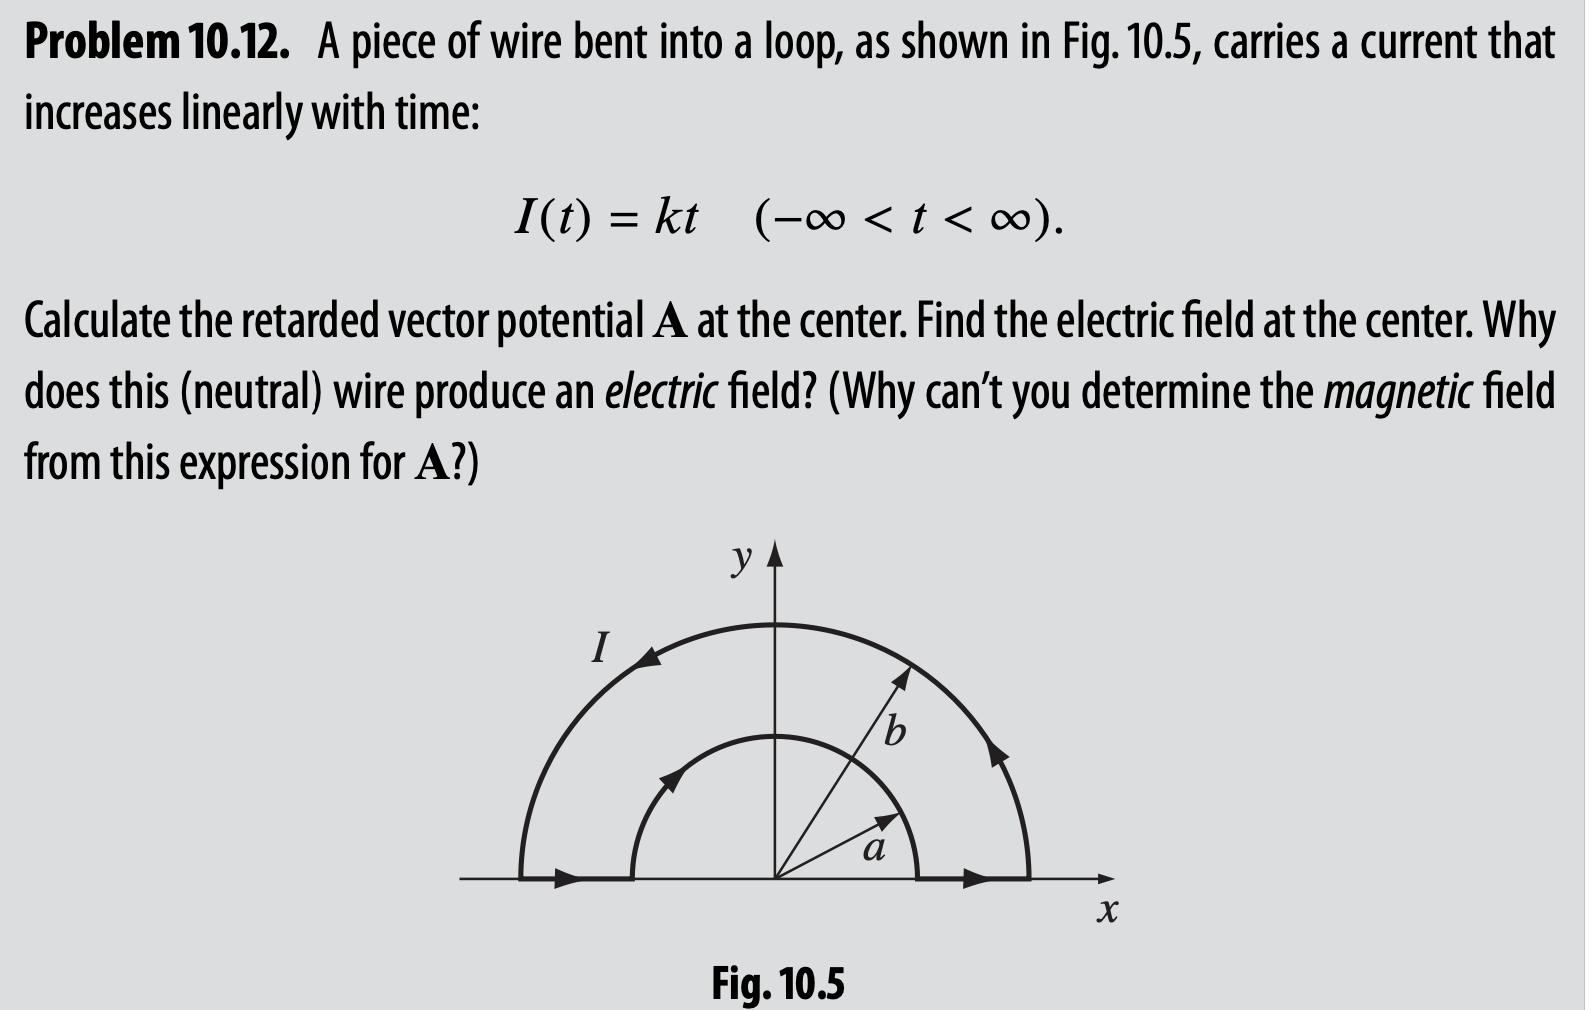
\includegraphics[width=0.8\textwidth]{Griffiths_prob_10_12.png}
\end{figure}

In general, the relevant one-dimensional integral is along the wire: \begin{align*}
    \mathbf{A}(\mathbf{r}, t) = \frac{\mu_0}{4 \pi } \int \frac{\mathbf{I}(\mathbf{r}^{\prime} , t_r)}{\griffr[2] } d l ^{\prime} 
\end{align*}

But the current only depends on time and not on position. Along the top wire we get \begin{align*}
    \mathbf{I}(t_r) = k(t - \frac{b}{c})\hat{\boldsymbol{\phi}} = (t - \frac{b}{c})\left[ - \sin \theta \hat{\mathbf{x}} + \cos \theta \hat{\mathbf{y}} \right] 
\end{align*}
while along the bottom we have \begin{align*}
    \mathbf{I}(t_r) = k(t - \frac{a}{c})(-\hat{\boldsymbol{\phi}}) = (t - \frac{a}{c})\left[ \sin \theta \hat{\mathbf{x}} - \cos \theta \hat{\mathbf{y}} \right] 
\end{align*}
such that from those contributions we get \begin{align*}
    \mathbf{A}_{\text{top and bottom}}(\mathbf{r}, t) = \frac{k\mu_0}{4 \pi } \biggl[ &\hat{\mathbf{x}} \int_0 ^\pi  d \theta \sin \theta \left( a\left( t- \frac{a}{c} \right) +  b\left(t - \frac{b}{c}\right) \right)\\
      &\hat{\mathbf{y}} \int_0 ^\pi d \theta \cos \theta \left( b \left( t - \frac{b}{c} \right) + a \left( t - \frac{a}{c} \right)   \right) \biggr]
\end{align*}
plenty of things are independent of \(\theta \) so we get \begin{align*}
    \mathbf{A}_{\text{top and bottom}}(\mathbf{r}, t) = \frac{k\mu_0}{2\pi } \left( t (a + b) -  \frac{1}{c}\left( a^{2} + b^{2}  \right) \right) 
\end{align*}
whereas from the horizontal segments we get (I think they will be equal, but the "doppler" effect would actually play in here with a point charge. This is why we have terms involving the velocity vector in that case. But here I think they should be the same in the sense that it is symmetrical w.r.t.\ time):
\begin{align*}
    \mathbf{A}_{\text{left horizontal}}(\mathbf{r}, t) &= \frac{k\mu_0}{4 \pi } \hat{\mathbf{x}} \int_b ^a \frac{t - \frac{x^{\prime}}{c} }{x^{\prime}} dx^{\prime} \\
    &=  \frac{k\mu_0}{4 \pi } \hat{\mathbf{x}} \left( t \ln \left(\frac{a}{b}\right) - \frac{a - b}{c} \right) 
\end{align*}
but of course with the right horizontal, we are integrating the exact same thing, but from \(a \to  b\). Thus they cancel. This seems wierd to me right now, since with the right hand rule from the current, I would think the field would have to contribute something. But I do see that the center is on the line of the two horizontal segments. But if we only had one side, that should prevent the field, right? I got a contribution from the left side alone. It was just cancelled by the right side it seems.  

\subsection*{Follow-Up Questions/Ideas/ToDos}
\begin{itemize}
    \item It seems weird that there can be different retarded times from the same field point to a point charge, but that's apparently necessary with classical electrodynamics. \textred{What's the full story?}
    \item In problem 10.12 above, it confuses me that flipping the limits of integration is the same as flipping the direction of the current in some sense. When we are running along the inner half circle (the one at radius \(a\)), I have the urge to say that it is running in the direction \(- \boldsymbol{\hat{\mathbf{\phi}}}\) while the angle being sweeped is from \(\pi \to 0\). But this is "a double flip" and leaves the integral unchanged. At the same time, I feel like the two horizontal wire segments shouldn't cancel. They are running in the same direction one would think. But with respect to the center point, they \textit{are} running in oppositse directions of course.  
\end{itemize}


\end{document}
